% Slides 11--12: rolling annual cross-validation and interpretation.

\begin{frame}{Annual performance is tested out of sample}
  \begin{columns}[T,onlytextwidth]
    \begin{column}{0.54\textwidth}
      \begin{enumerate}
        \item Hold out four consecutive years
        \item Fit frequency and severity models on the remaining years
        \item Predict aggregate payout for the held-out years
        \item Move the holdout block through 2010--2025
      \end{enumerate}

      Both model components are evaluated together on observations
      not used for fitting.
    \end{column}
    \begin{column}{0.40\textwidth}
      \textbf{Example split}

      \begin{itemize}
        \item 2010--2021: model fitting
        \item 2022--2025: held out
        \item Output: annual total payout
      \end{itemize}

      \vspace{0.45cm}
      Final projections use models fitted to all 16 years.
    \end{column}
  \end{columns}
  \sourceNote{Rolling block cross-validation, Gjensidige 2010--2025}
\end{frame}

\begin{frame}{The model tracks the trend, not every extreme year}
  \begin{columns}[T,onlytextwidth]
    \begin{column}{0.38\textwidth}
      \begin{itemize}
        \item Broad rises and falls are captured
        \item Some individual years have substantial level errors
        \item The 2023 prediction is almost one period mean below the
          observation
        \item No comparable ``Hans year'' remains when 2023 is held out
      \end{itemize}

      \textbf{Intended use:} long-period aggregate change, not
      individual-year prediction.
    \end{column}
    \begin{column}{0.59\textwidth}
      % Replace with the English-labelled plot using the same filename.
      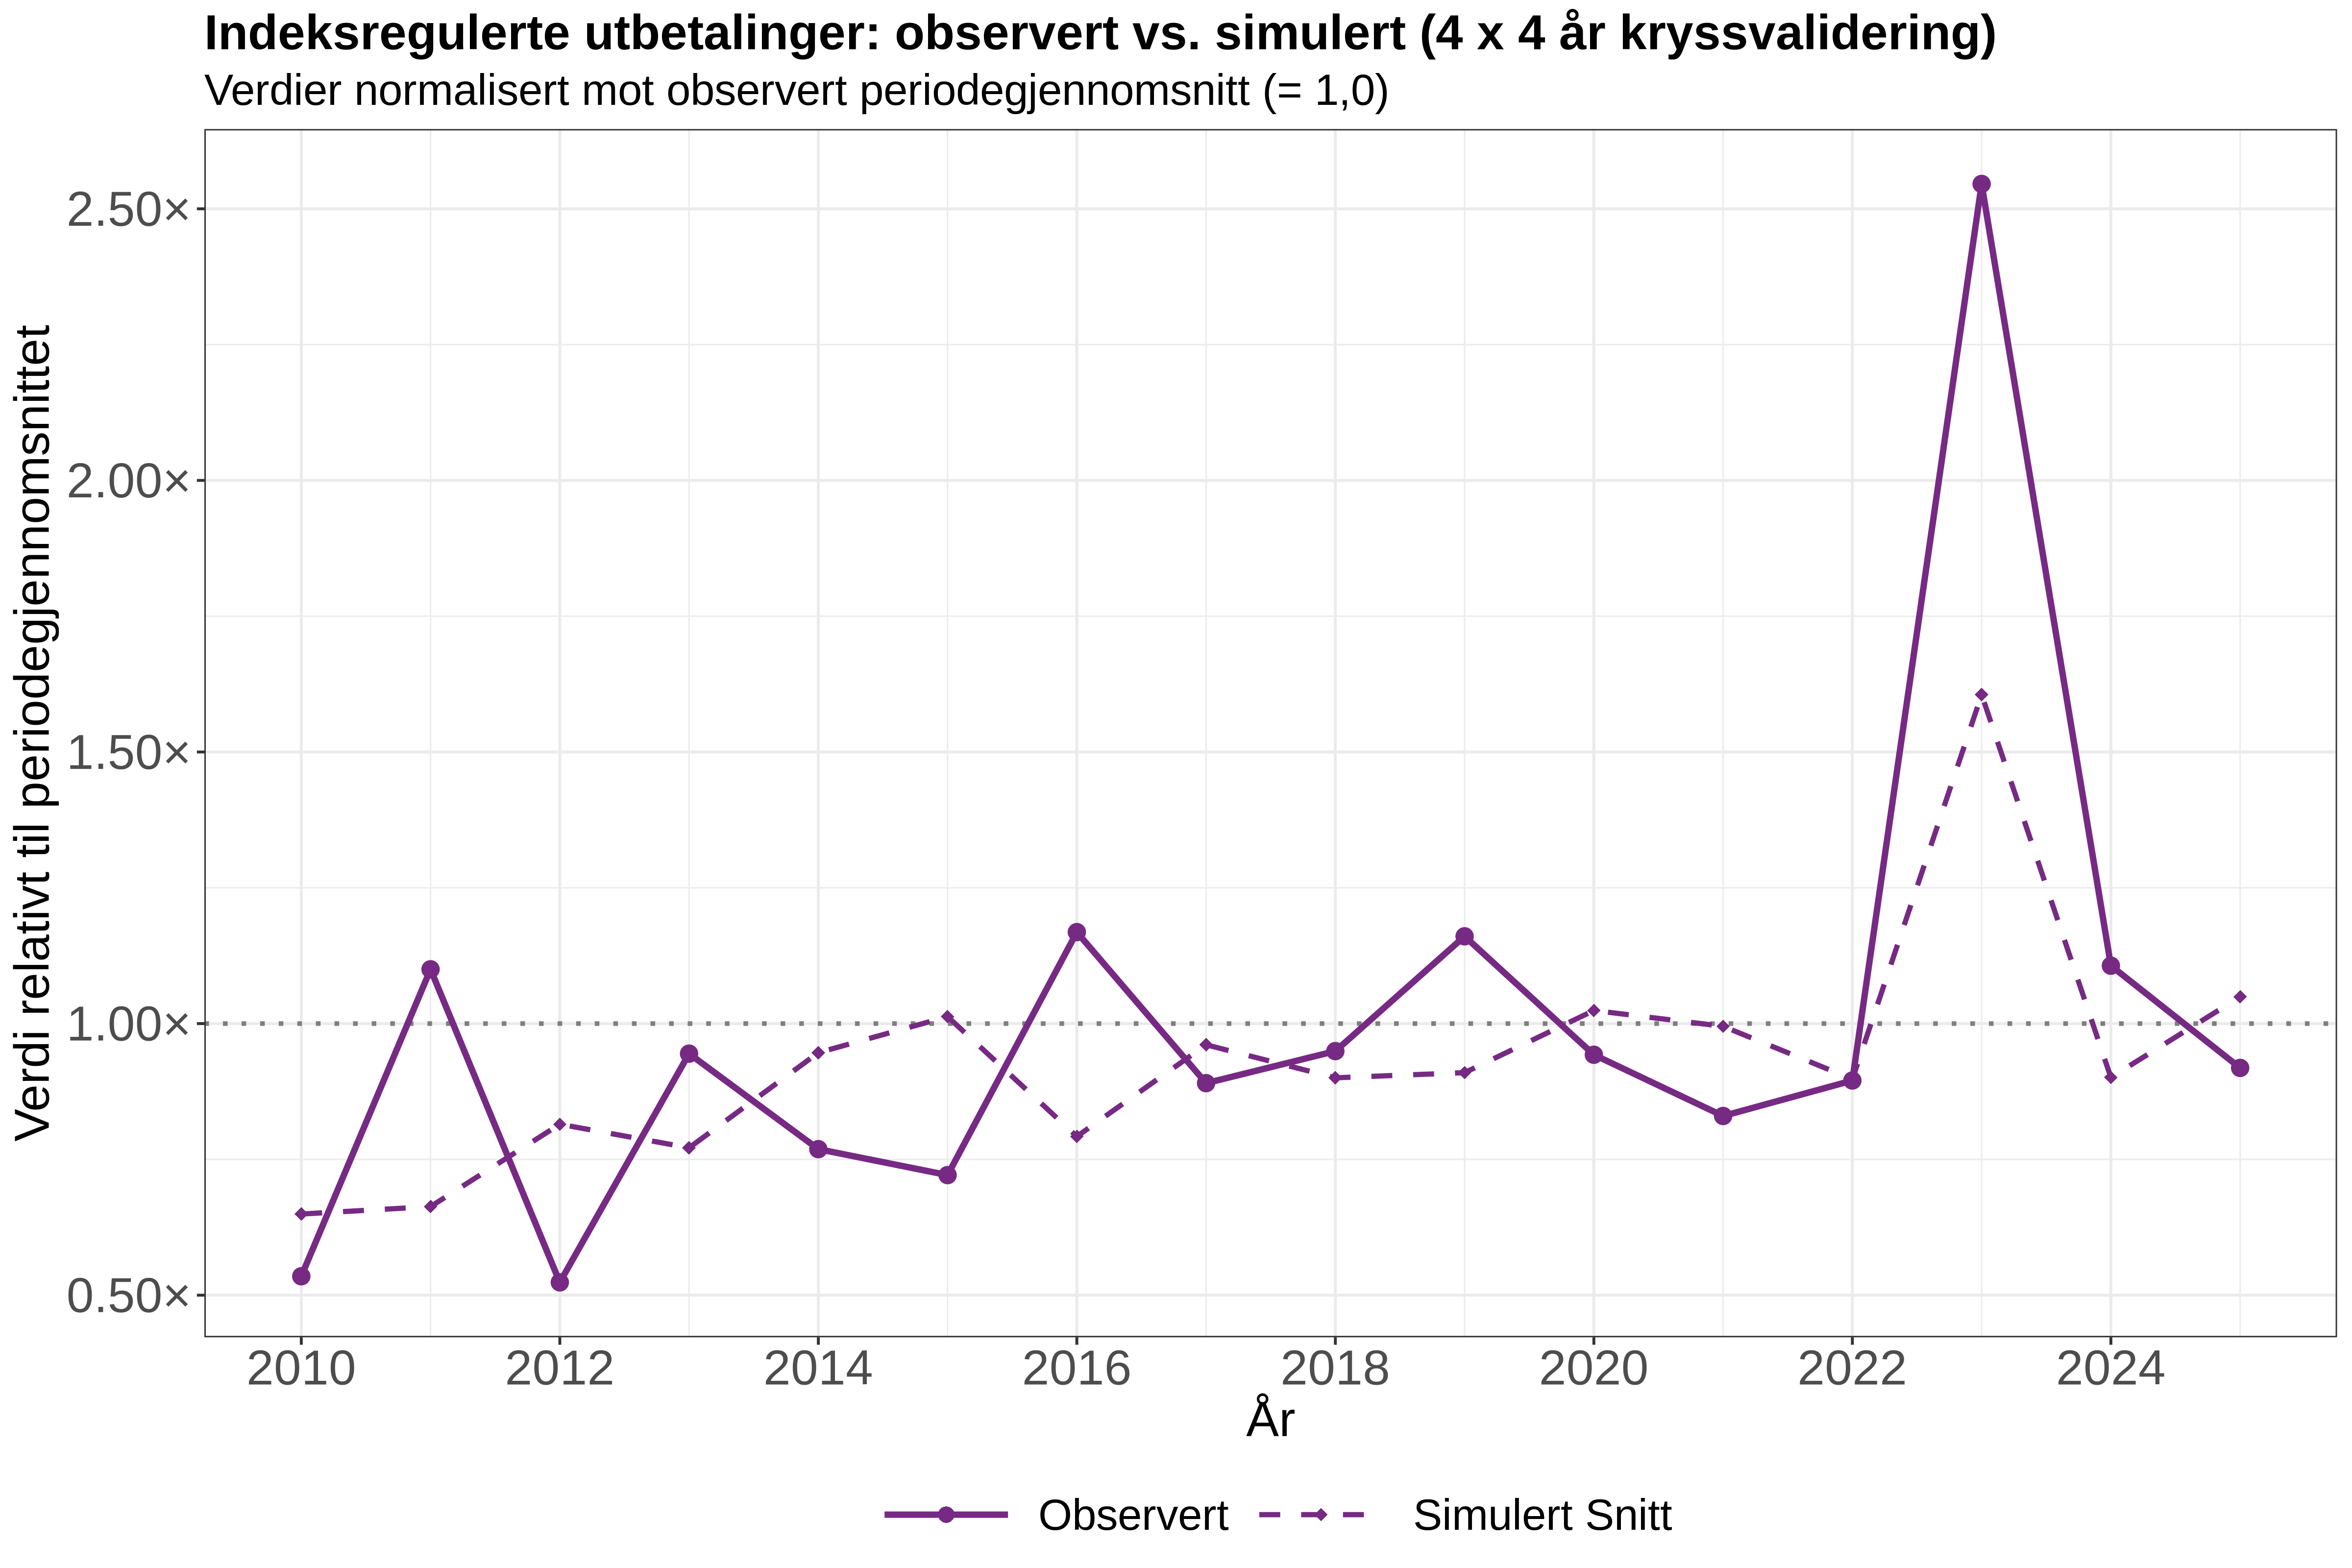
\includegraphics[width=\linewidth,height=0.50\textheight,keepaspectratio]{images/cross-validation.png}
    \end{column}
  \end{columns}
  \sourceNote{Four-year rolling cross-validation; annual payouts
  normalised by exposure}
\end{frame}
